% JuliaCon proceedings template
\documentclass{juliacon}
\setcounter{page}{1}

\usepackage{xspace}

\usepackage{subcaption}

\usepackage{hyperref}

\hypersetup{colorlinks=true,linkcolor=blue,urlcolor=blue}

\newcommand{\ie}{\emph{i.e.}}
\newcommand{\cp}{\textsc{CP}\xspace}
\newcommand{\csp}{\textsc{CSP}\xspace}
\newcommand{\cop}{\textsc{COP}\xspace}
\newcommand{\efsp}{\textsc{EFSP}\xspace}
\newcommand{\efop}{\textsc{EFOP}\xspace}
\newcommand{\cfn}{\textsc{CFN}\xspace}
\newcommand{\wcsp}{\textsc{WCSP}\xspace}
\newcommand{\cbls}{\textsc{CBLS}\xspace}
\newcommand{\ghost}{\textsc{GHOST}\xspace}
\newcommand{\cppn}{\textsc{CPPN}\xspace}
\newcommand{\icn}{\textsc{ICN}\xspace}

\newcommand{\jc}{\href{https://github.com/JuliaConstraints}{JuliaConstraints}\xspace}
\newcommand{\cdjl}{\href{https://github.com/JuliaConstraints/ConstraintDomains.jl}{ConstraintDomains.jl}\xspace}
\newcommand{\cnjl}{\href{https://github.com/JuliaConstraints/CompositionalNetworks.jl}{CompositionalNetworks.jl}\xspace}
\newcommand{\cjl}{\href{https://github.com/JuliaConstraints/Constraints.jl}{Constraints.jl}\xspace}
\newcommand{\cmjl}{\href{https://github.com/JuliaConstraints/ConstraintModels.jl}{ConstraintModels.jl}\xspace}
\newcommand{\lssjl}{\href{https://github.com/JuliaConstraints/LocalSearchSolvers.jl}{LocalSearchSolvers.jl}\xspace}
\newcommand{\cblsjl}{\href{https://github.com/JuliaConstraints/CBLS.jl}{CBLS.jl}\xspace}


\newcommand{\cproblem}[3]%
{\begin{trivlist}
  \item[]%
    \textbf{Problem:} \textsc{#1}\\
    \textit{Input:} #2\\
    \textit{Question:} #3
  \end{trivlist}%
}

\begin{document}

% **************GENERATED FILE, DO NOT EDIT**************

\title{CompositionalNetworks.jl: a scaling glass-box neural network to learn combinatorial functions}

\author[1]{Jean-François \textsc{Baffier}}
\author[2]{Khalil \textsc{Chrit}}
\author[3,4]{Florian \textsc{Richoux}}
\author[2]{Pedro \textsc{Patinho}}
\author[2]{Salvador \textsc{Abreu}}
\affil[1]{IIJ, Japan}
\affil[2]{NOVA-LINCS, University of Évora, Portugal}
\affil[3]{AIST, Japan}
\affil[4]{JFLI, CNRS, Japan}

\keywords{Julia Language, Constraint Programming, Local Search, Metaheuristics, Neural Network, Metaprogramming, Scalable Machine Learning, Glass-Box Algorithm}

\hypersetup{
pdftitle = {CompositionalNetworks.jl: a scaling glass-box neural network to learn combinatorial functions},
pdfsubject = {JuliaCon 2019 Proceedings},
pdfauthor = {Jean-François \textsc{Baffier}, Khalil \textsc{Chrit}, Florian \textsc{Richoux}, Pedro \textsc{Patinho}, Salvador \textsc{Abreu}},
pdfkeywords = {Julia Language, Constraint Programming, Local Search, Metaheuristics, Neural Network, Metaprogramming, Scalable Machine Learning, Glass-Box Algorithm},
}



\maketitle

\begin{abstract}
  Interpretable Compositional Networks (ICNs) are a neural network variant for combinatorial function learning that allows the user to obtain interpretable results, unlike ordinary artificial neural networks. An ICN outputs a composition of functions that scale with the size of the input, allowing a learning phase on relatively small spaces.
  \cnjl is a pure Julia package that exploits the language's meta-programming, parallelism and multiple dispatch features to produce learned compositions in mathematical and programming languages such as Julia, C or C++.
\end{abstract}

\section{Introduction}
\label{sec:introduction}

The discipline of combinatorial optimization consists in finding an optimal configuration of elements within a finite set. Such a set is usually subject to constraints that can be represented by functions that are often highly combinatorial. These constraints are mostly formulated as concepts, boolean functions indicating whether each constraint is respected or not. A solution (sometimes called a satisfactory solution, depending on the domain) is a configuration that respects all the constraints.

Different domains such as operational research, constraint programming, metaheuristics, propose methods to find (satisfactory or optimal) solutions. Among these methods, some can or could benefit from a finer granularity in the evaluation of the impact of each constraint on a given configuration.

In \cite{richoux2020automatic}, we introduced Interpretable Compositional Networks (ICNs), a neural network variant for combinatorial function learning that allows the user to obtain interpretable results, unlike ordinary artificial neural networks. An ICN outputs a composition of functions that scale with the size of the input, allowing a learning phase on relatively small spaces.

This work, consists in a library that implements ICNs in the Julia programming language \cite{bezanson2017julia}. Although we present a direct application of ICNs in the following subsection, this neural network framework is simple to extend to learn other combinatorial and non-combinatorial functions.

\subsection{Application to Constraint Programming}
\label{subsec:cpcontext}

Constraint Satisfaction Problem (\csp) and Constrained Optimization Problem (\cop) are constraint-based problems where constraints can be seen as predicates (\emph{concepts}) allowing or forbidding some combinations of variable assignments.
Such a formulation corresponds well to the so-called complete solution methods which guarantee an exploration of all solutions. Unfortunately, due to the highly combinatorial nature of some problems, these methods cannot always converge in a reasonable time.

\begin{figure}[t]
  \centerline{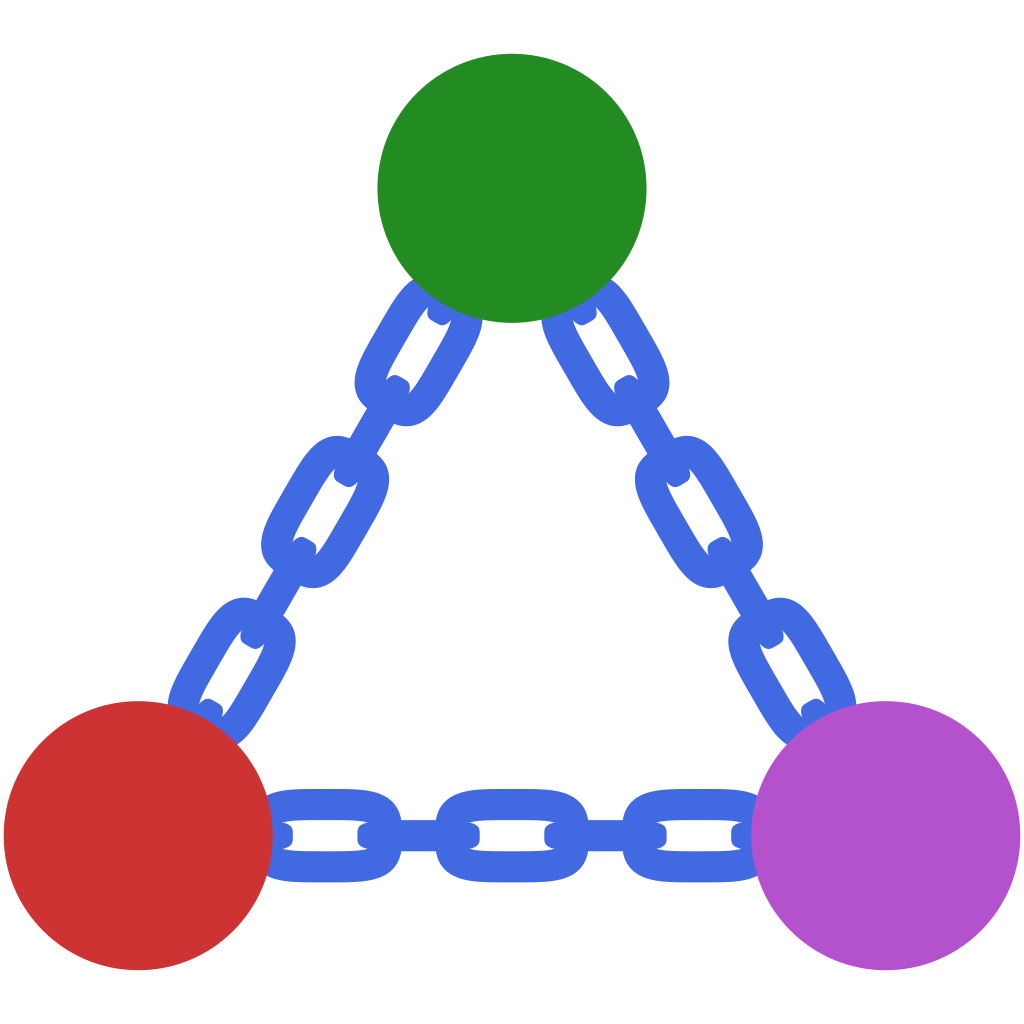
\includegraphics[width=5cm]{figs/juliaconstraints.png}}
  \caption{Logo of the \jc organization on GitHub that hosts, among other things, the \cnjl package.}
  \label{fig:juliaconstraints}
\end{figure}

On the other hand, Constraint-Based Local Search (\cbls) is a family of metaheuristics in which the neighborhood is constructed on the basis of an \emph{error function}, itself a quantitative representation of how far the current configuration is from an admissible solution. We refer to the corresponding problems as Error Function Satisfaction Problem (\efsp) and Error Function Optimization Problem (\efop). In the case of \cbls, this is computed as a function of the constraints which are not currently satisfied. Error functions may be derived from the constraint satisfaction problem structure, hand-coded, automatically acquired by some machine learning process, or constructed as a combination of these methods. It should be noted that, the best performing systems resort to hand-tuned error functions, as witness~\cite{DBLP:books/sp/18/CodognetMDA18}.

As illustrated by Figure~\ref{fig:landscape}, a well-designed error function helps in converging faster towards better-quality solutions.  It does, however, introduce an additional layer of complexity to the user.

\begin{figure}[t]
  \centering
  \subcaptionbox{CSP landscape\label{sfig:csp}}{
    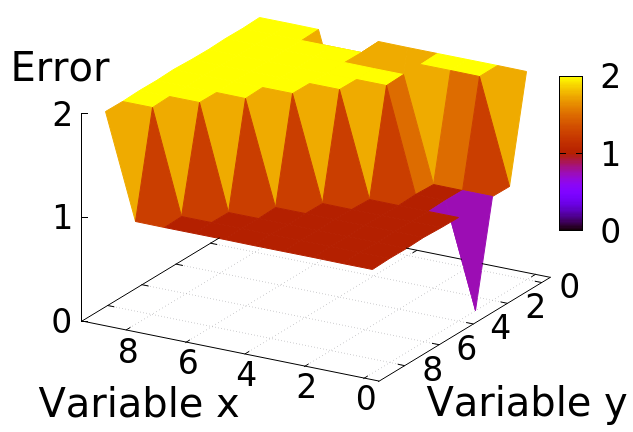
\includegraphics[width = .95\columnwidth]{figs/csp_landscape_complex_zero_big.png}
  }

  \subcaptionbox{EFSP landscape\label{sfig:efsp}}{
    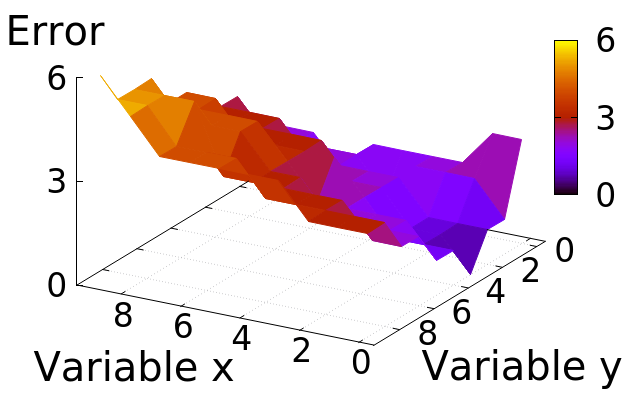
\includegraphics[width = .95\columnwidth]{figs/efsp_landscape_complex_zero_big.png}
  }\caption{
    Comparison of a Constraint Satisfaction Problem (CSP) and an Error
    Function Satisfaction Problem (\efsp) landscapes. The finer scale
    in the error heuristic of the \efsp leads to a better convergence
    rate.}\label{fig:landscape}
\end{figure}

\subsection{Interpretable Compositional Networks (ICN)}
\label{subsec:icn}

In \cite{richoux2020automatic}, we proposed a neural network inspired by Compositional Pattern-Producing Networks (\cppn) to learn (highly) combinatorial functions as non-linear combinations of elementary operations. \(\cppn\)s~\cite{stanley2007cppn} are themselves a variant of artificial neural networks. While neurons in regular neural networks usually  contain sigmoid-like functions only (such  as ReLU, \ie{} Rectified Linear  Unit), \cppn's neurons can contain many other kinds of functions: sigmoids, Gaussians, trigonometric functions, and linear functions among others.
\(\cppn\)s are often used to generate 2D or 3D images by applying the function modeled by a \cppn giving each pixel individually as input, instead of considering all pixels at once. This simple trick allows the learned \cppn model to produce images of any resolution.

We propose our variant by taking these two principles from \cppn: having neurons containing one operation among many possible ones, and handling inputs in a size-independent fashion. Due to their interpretable nature, we named our variant \textbf{Interpretable Compositional Networks} (\icn).

Although ICNs are not limited to learning function for \efsp/\efop, the original structure was designed to learn compositions weighted in accordance to the hamming metric \cite{richoux2020automatic}. The hamming distance between a configuration and its closest solution is a meaningful indicator of the number of variables needed to be changed. Manhattan and other variants of minkowski comparison are other example of possible metrics.

An ICN is made of several layers of (possibly exclusive) operations such that the first layers accept a vector as input and the last layer returns a single numerical value. Generally, layers alter there input in three possible ways: \emph{increment}, \emph{decrement}, or \emph{conservation} of the dimension of the input.

\begin{figure}[t]
  \centerline{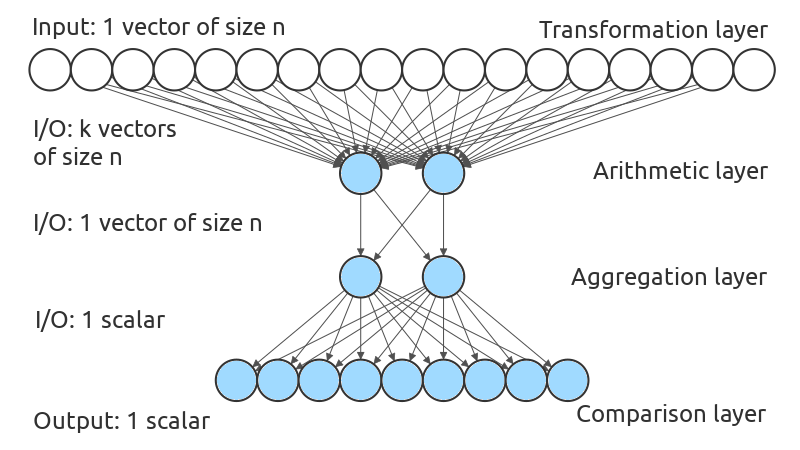
\includegraphics[width=\columnwidth]{figs/model_nn.png}}
  \caption{Scheme of the basic 4-layers ICN model used in \efsp/\efop. Layers with blue neurons have mutually exclusive operations. the \emph{transformation} layer increases the input dimension, the \emph{arithmetic} and \emph{aggregation} layers reduces it, and the \emph{comparison} layer leaves it untouched. The figure is taken from \cite{richoux2020automatic}.}
  \label{fig:model_icn}
\end{figure}

In the context of \efsp/\efop, the output should be non-negative if the constraint is violated and equal to 0 otherwise. As shown by Figure \ref{fig:model_icn}, our \(\icn\)s are
composed of four layers, each of them having a specific purpose and
themselves composed of neurons applying  a unique operation each.  All
neurons  from  a  layer  are  linked to  all  neurons  from  the  next
layer. The weight on each link is purely binary: its value is either 0
or 1. This restriction is  crucial to obtain interpretable functions. We refer the reader to \cite{richoux2020automatic} for a more comprehensive definition.

\subsection{A first C++ library}
\label{subsec:cplusplus}

In \cite{richoux2020automatic} we introduced the concept of ICN and a first implementation for Constraint Programming as a C++ library\footnote{\url{https://github.com/richoux/LearningUtilityFunctions}}. The results were evaluated through the GHOST C++ solver \cite{richoux2016ghost} and serve as a proof of concept that most of the models give scalable functions, and remain fairly effective using incomplete training sets.

As mentioned in Section \ref{sec:xlc}, \cnjl generates code for a direct use in Julia, but also exports usable code for both the GHOST(C++) and AdaptiveSearch (C)\footnote{This feature is a WIP at the moment this article is submitted, but is expected to be completed in the coming weeks.}. The code exported in C++, that is the \emph{operations} of each neuron, is strongly inspired by our C++ library.

\section{The example of the \jc framework}
\label{sec:juliaconstraints}

The \cnjl package is part of the \jc GitHub organization that proposes a first collection of Julia packages for Constraint-Based Local Search (CBLS), a subfield of Constraint Programming.

The main goal of this framework is to provide a set of high level semi-automatic tools which strike a good compromise between efficiency and ease of modeling.

\subsection{History of \jc}
\label{subsec:history}

The LocalSearchSolvers.jl package is a Constraint-Based Local Search framework started in Fall 2020 and inspired by other CBLS solvers such as GHOST (C++) and AdaptiveSearch (C) that allows users to tune their own solver.

During the development of LocalSearchSolvers.jl, we decided to split the code and functionality of the original framework into several independent packages for ease of maintenance and in hopes of providing common tools for other constraint programming packages in Julia.

During 2021, these tools were collected into the \jc ecosystem as follows
\begin{itemize}
  \item \cdjl: creation of discrete, continuous, and arbitrary domain (beta status)
  \item \cjl: generation of constraints from a boolean concept or an error function. Also list usual constraints and their properties (beta status)
  \item \cnjl: stable
  \item \lssjl: A CBLS framework in Julia with built-in parallel and distributed scalability
  \item \cblsjl: A MOI/JuMP wrapper for LocalSearchSolvers
  \item \cmjl: list of CP models for \cblsjl and \lssjl
\end{itemize}

\begin{figure*}[t]
  \centerline{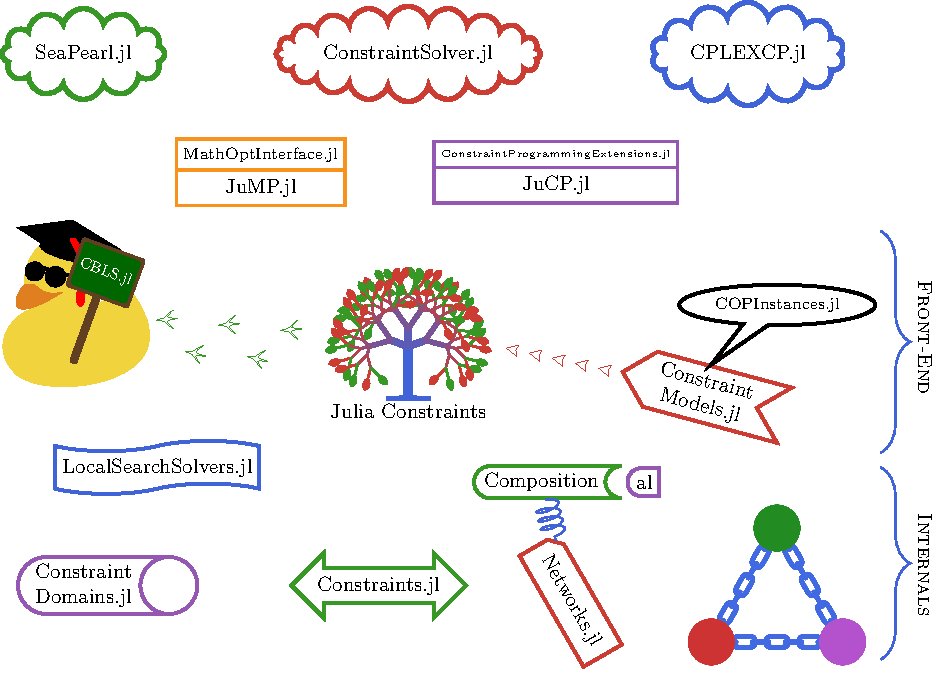
\includegraphics[page=1, width=.9\textwidth]{figs/overview.pdf}}
  \caption{Overview of the Constraint Programming ecosystem in Julia, including \jc. \emph{Front-End} and \emph{Internals} refer to the latest. Note that, at the moment of the writing, \texttt{ConstraintProgrammingExtension.jl}, \texttt{JuCP.jl}, and \texttt{COPInstances.jl} are temporary names.}
  \label{fig:overview}
\end{figure*}

The global state of the Constraint Programming ecosystem is presented in Figure \ref{fig:overview}. Beside the CBLS framework of \jc, other solvers are complete search methods, such as ConstraintSolver.jl\footnote{\url{https://github.com/Wikunia/ConstraintSolver.jl}}, CPLEXCP.jl\footnote{\url{https://github.com/dourouc05/CPLEXCP.jl}}, and SeaPearl.jl \cite{chalumeau2021seapearl}.

\subsection{A simple example with \texttt{CBLS.jl}}
\label{subsec:example}

A Magic Square of order $n$ is composed of $n^2$ distinct values ranging from $1$ to $n^2$ layed out as a square array $X$.  These values need to be arranged such that the sums of each diagonal, row and column be equal to the same value, the magic sum $\Sigma$.

\[ \sum_{j=1}^{n} X_{ij} = \sum_{i=1}^{n} X_{ij} = \sum_{j=1}^{n} X_{ii} = \sum_{j=1}^{n} X_{i,n-i+1} = \frac{n(n^{2}+1)}{2} = \Sigma \]

\begin{figure}[t]
  \centerline{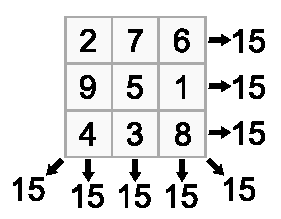
\includegraphics[page=1]{figs/magicsquare.pdf}}
  \caption{A solved magic-square of size $3$. The \emph{magic sum} is equal to $15$. Image from Wikipedia's user \textsc{Phidauex}.}
  \label{fig:magicsquare}
\end{figure}

In \texttt{ConstraintModels.jl}, we use the following code to generate a magic-square instance.

\begin{lstlisting}[language = Julia]
# Import CBLS.jl and JuMP.jl
using CBLS, JuMP

function magic_square(n::Integer)
model = Model(CBLS.Optimizer)
N = n^2
Σ = n * (N + 1) / 2
@variable(model, 1 <= X[1:n, 1:n] <= N, Int)
@constraint(model, vec(X) in AllDifferent())
for i in 1:n
  @constraint(model, X[i,:] in Linear(Σ))
  @constraint(model, X[:,i] in Linear(Σ))
end
@constraint(model,
  [X[i,i] for i in 1:n] in Linear(Σ)
)
@constraint(model,
  [X[i,n+1-i] for i in 1:n] in Linear(Σ)
)
  return model, X
end

# Create a magic square instance of size 4x4
m, X = magic_square(4)
# Optimize
optimize!(m)
# Output values
@info values.(X)
\end{lstlisting}

\section{A flexible implementation}
\label{sec:implementation}

\cnjl extends the work of the first C++ library used in \cite{richoux2020automatic}. As mentioned in Section \ref{subsec:cplusplus}, that library used for prototyping was limited through several aspects: this, this, and that. Obviously, those limitations could have been lifted in the first library. However, we decided to use some features of the Julia language to ease provisioning flexibility and broader features to ICNs.

\paragraph*{Block about Julia} test

\subsection{Layers of operations}
\label{subsec:layers}

A layer is defined by a non-empty collection of (possibly mutually exclusive) operations. The original ICN is composed of four layers: \emph{transformation} (exclusive), \emph{arithmetic}, \emph{aggregation}, and \emph{comparison}.

\begin{lstlisting}[language = Julia]
struct Layer
  functions::LittleDict{Symbol, Function}
  exclusive::Bool
end
\end{lstlisting}

\begin{lstlisting}[language = Julia]
# Transformation defined for a vector
tr_identity(x; param=nothing) = identity(x)

# Transformation defined for the index of a vector
tr_count_eq(i, x; param=nothing) =
  count(y -> x[i] == y, x) - 1
tr_count_eq_param(i, x; param) =
  count(y -> y == x[i] + param, x)

# Generating vectorized versions
lazy(tr_count_eq)
lazy_param(tr_count_eq_param)
\end{lstlisting}

\begin{lstlisting}[language = Julia]
function transformation_layer(param=false)
  transformations = LittleDict{Symbol,Function}(
    :identity => tr_identity,
    :count_eq => tr_count_eq,
    # ...
  )
  if param
    tr_param = LittleDict{Symbol, Function}(
      :count_eq_param => tr_count_eq_param,
      # ...
    )
    transformations = LittleDict(
      union(transformations, tr_param)
    )
  end
  return Layer(transformations, false)
end
\end{lstlisting}

All methods required for the definition of additional layers are all available.

\subsection{Composition}
\label{subsec:composition}

We store the composition of an ICN in three forms:
\begin{itemize}
  \item A collection of \texttt{Symbol}s per layer of the ICN that allows the generation of code as a string
  \item The Julia object of type \texttt{Function} to apply the composition directly
\end{itemize}

\begin{lstlisting}[language = Julia]
struct Composition{F<:Function}
  code::Dict{Symbol,String}
  f::F
  symbols::Vector{Vector{Symbol}}
end
\end{lstlisting}

The result output by an ICN is a composition, a mathematical function composed of several basic operations. The \texttt{code} function returns the definition of a composition in either a mathematical or programming language. From \emph{v1.0} of \cnjl, \texttt{code} accepts \texttt{:maths, :Julia, :C, :Cpp} as values for the \emph{lang} key argument.

\begin{lstlisting}[language = Julia]
function code(
  c::Composition, lang=:maths;
  name="composition"
)
  return get!(
    c.code, lang, generate(c, name, Val(lang))
  )
end
\end{lstlisting}

\section{Explore, learn, and compose}
\label{sec:xlc}

It is far from practical to apply the internals of \cnjl step-by-step. We provide a user-friendly sequence of higher-level actions, \emph{explore}, \emph{learn}, and \emph{compose} that fits most of expected uses of this package.

Each of those actions is semi-automated through default parameters and machine learning over a large collection of benchmarks \cite{baffier2022interpretable}.

\subsection{Exploration}

\begin{lstlisting}[language = Julia]
function explore(
  domains,
  concept,
  param=nothing;
  search=:flexible,
  complete_search_limit=10^6,
  max_samplings=sum(domain_size, domains),
  solutions_limit=floor(Int, sqrt(max_samplings)),
)
  if search == :flexible
    search = sum(domain_size, domains) <
      complete_search_limit ? :complete : :partial
  end
  return explore(Val(search), domains, concept,
    param, solutions_limit, max_samplings
  )
end
\end{lstlisting}



\section{Future challenges}
\label{sec:future}

\begin{itemize}
  \item Add new operations in existing layers
  \item Add new layers
  \item Use reinforcement learning
  \item Cover more metrics
  \item Apply ICN to other field than EFN for CBLS solvers
\end{itemize}

\section{Problems, constraints, and compositions zoo}
\label{sec:zoo}

The problems modelled, and the compositions extracted in this section are subject to future changes and improvements of the JuMP/JuCP packages. However, the keys ideas are presented here and examples will be updated accordingly within \jc in the future.

\subsection{A few combinatorial models}
\label{subsec:models}

\begin{lstlisting}[language = Julia]
function mincut(graph, source, sink, interdiction)
  m = JuMP.Model(CBLS.Optimizer)
  n = size(graph, 1)
  separator = n + 1

  @variable(m, 0 <= X[1:separator] <= n, Int)

  @constraint(m,
    [X[source], X[separator], X[sink]] in Ordered()
  )
  @constraint(m, X in AllDifferent())

  obj(x...) = o_mincut(graph, x...; interdiction)
  @objective(m, Min, ScalarFunction(obj))

  return m, X
end
\end{lstlisting}

\begin{lstlisting}[language = Julia]
function golomb(n, L)
  m = JuMP.Model(CBLS.Optimizer)

  @variable(m, 0 <= X[1:n] <= L, Int)

  @constraint(m, X in AllDifferent())
  @constraint(m, X in Ordered()) # optional

  # No two pairs have the same length
  for i in 1:(n - 1), j in (i + 1):n
    for k in i:(n - 1), l in (k + 1):n
      (i, j) < (k, l) || continue
      @constraint(m,
        [X[i], X[j], X[k], X[l]] in DistDifferent()
      )
    end
  end

  # Add objective
  @objective(m, Min, ScalarFunction(maximum))

  return m, X
end
\end{lstlisting}

\subsection{Constraints and compositions}
\label{subsec:constraints}

Along with the magic-square model in Section \ref{sec:introduction}, the models in this zoo use the following constraints: \texttt{:all\_different}, \texttt{:dist\_different}, \texttt{:linear}, and \texttt{:ordered}.

The \emph{AllDifferent} constraint ensures that all the values of a given configuration are unique.

\begin{lstlisting}[language = Julia]
function all_different(x;
  X = zeros(length(x), 1), param=nothing, dom_size
)
  tr_in(Tuple([tr_count_eq_left]), X, x, param)
  for i in 1:length(x)
    X[i,1] = ar_sum(@view X[i,:])
  end
  return ag_count_positive(@view X[:,1]) |> (
      y -> co_identity(
        y; param, dom_size, nvars=length(x)
      )
    )
end
\end{lstlisting}

\emph{DistDifferent} is constraint ensuring that \(|x[1] - x[2]| \neq |x[3] - x[4]|\) for any vector $x$ of size $4$.

\begin{lstlisting}[language = Julia]
function dist_different(x)
  return abs(x[1] - x[2]) != abs(x[3] - x[4])
end
\end{lstlisting}

\emph{Linear} (also called \emph{Sum} or \emph{LinearSum} in the literature) Global ensures that the sum of the values of $x$ is equal to a given parameter $param$. Note that this version is a simplification of a linear sum of values with some coefficients.

\begin{lstlisting}[language = Julia]
function linear(x; param, dom_size)
  return abs(sum(x) - param) / dom_size
end
\end{lstlisting}

\emph{Ordered} is a constraint ensuring that all the values of $x$ are ordered (here in a decreasing order).

\begin{lstlisting}[language = Julia]
function ordered(x;
  X = zeros(length(x), 1), param=nothing, dom_size
)
  tr_in(
    Tuple([tr_contiguous_vals_minus]), X, x, param
  )
  for i in 1:length(x)
    X[i,1] = ar_sum(@view X[i,:])
  end
  return ag_count_positive(@view X[:,1]) |> (
      y -> co_identity(
        y; param, dom_size, nvars=length(x)
      )
    )
end
\end{lstlisting}

\section{Acknowledgements}
\label{sec:acknowledgements}

We're grateful to Ricardo \textsc{Rosa} and Pranshu \textsc{Malik} for the logo of \jc presented as Figure \ref{fig:juliaconstraints}.

% **************GENERATED FILE, DO NOT EDIT**************

\bibliographystyle{juliacon}
\bibliography{ref.bib}


\end{document}

% Inspired by the International Journal of Computer Applications template
